\chapter{Introduction}
\label{cha:introduction}


\section{Motivation}

\begin{center}
    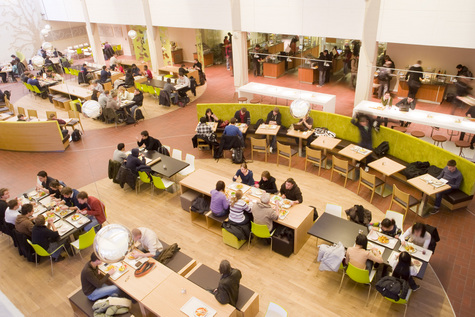
\includegraphics[width=\textwidth]{mensa}\\
    The mensa in Hardenbergstraße at TU Berlin.
\end{center}

Probably every person who has ever been to a mensa around lunch time will know the problem our project was about. You are hungry and your colleagues are too. Therefore in a group of maybe four people you enter the mensa and immediately start to spread out. Everyone likes a different dish, also some queues take longer than others and cash desks work after their own rhythm anyway. The result is: Finally done with paying for your food and in joyful anticipation of your deserved lunch you realize that at this point you don't have any clue anymore, where everyone went. Your colleagues all were faster than you but still managed to get away from the cash desks at different times and all started to look out for a place to sit with four people. This could look something like what the following graphic illustrates:

\begin{center}
    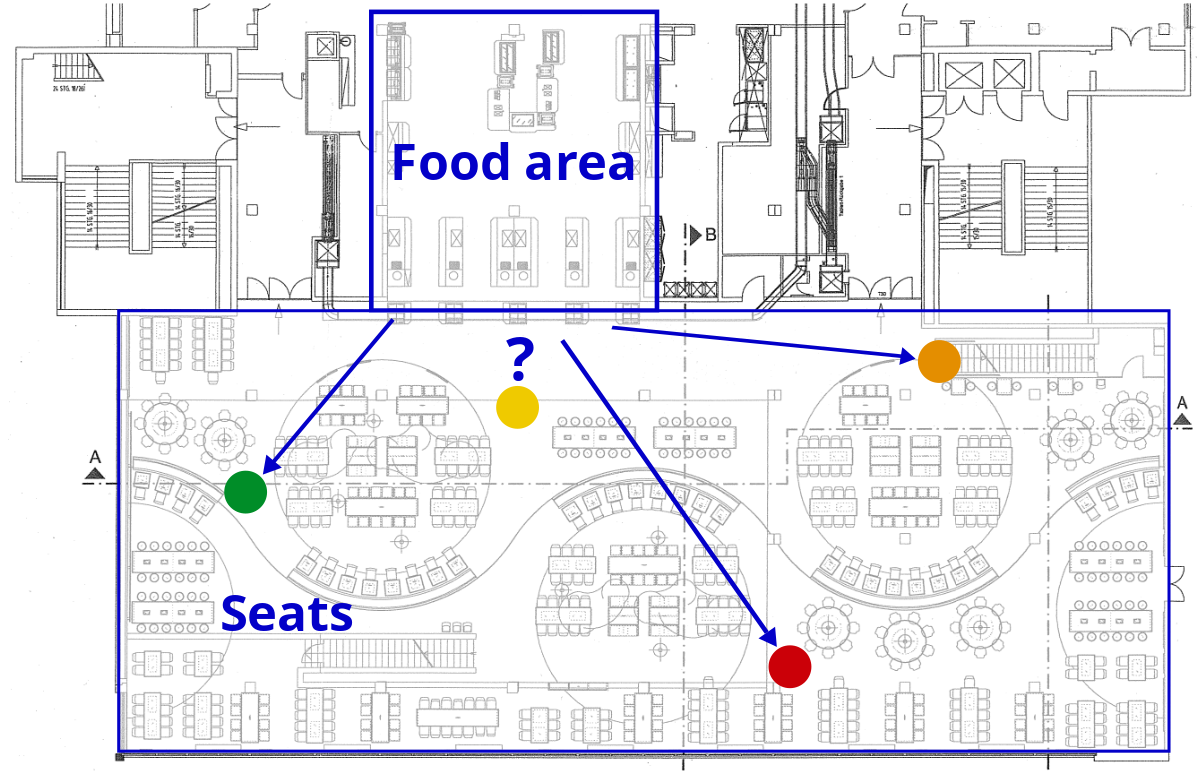
\includegraphics[width=\textwidth]{use-case-mensa-people}\\
    Yellow person looking for her/his friends in crowded mensa.
\end{center}

The same situation can happen in other big, crowded places where people try to meet as a group. As such, an example could be an university library in examination weeks where maybe a few people want to meet in order to study for their exams or even simply later want to have lunch in the mensa and experience the problem a second time. Either situation, exactly this problem of finding your peers in a user- yet privacy-friendly manner with modern hardware is the problem our project was focused to solve on.

As just mentioned, our project tackled this problem from a technological perspective. After all, we were part of the \enquote{Internet of Services Lab} (IoSL)\footnote{\url{https://www.snet.tu-berlin.de/menue/teaching/winter_term_2015_2016/internet_of_services_lab_wt20152016/}}, a project by the SNET department at TU Berlin. At the beginning of the semester we were brainstorming while preparing slides for the Milestone Workshop and we came up with the following vision of how our to-be-developed system should look like to an user:

\begin{center}
    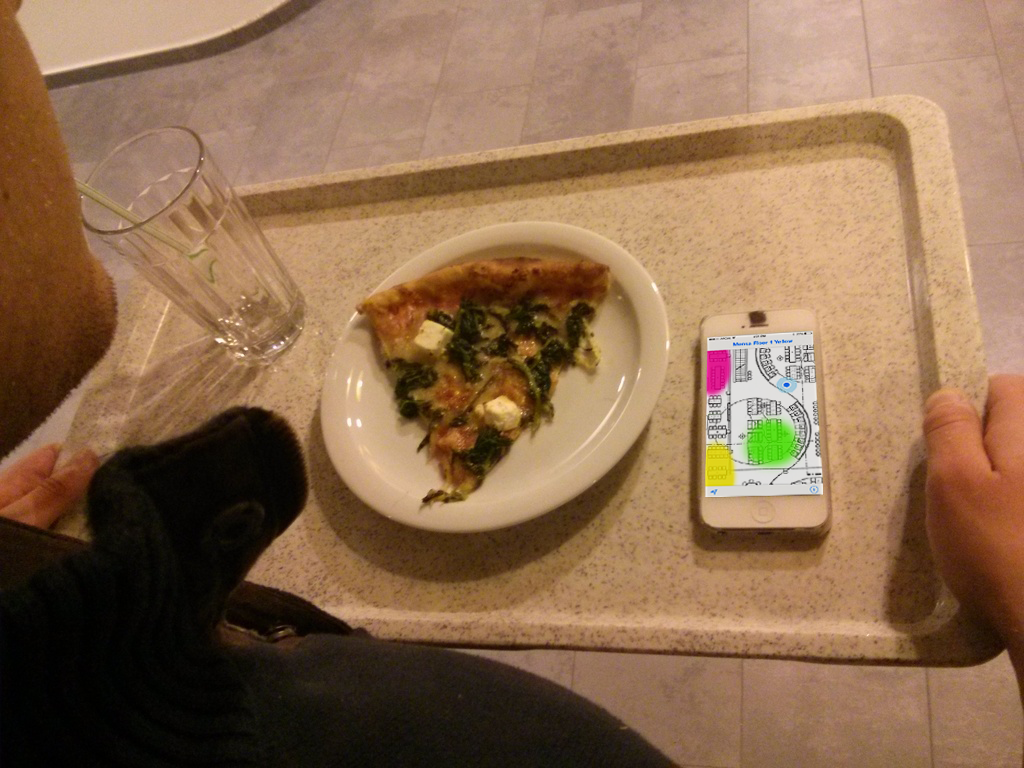
\includegraphics[width=\textwidth]{use-case-tablet}\\
    Imagined use of our app on a mensa tray.
\end{center}

The use of a smartphone was quite clear and of course, to interconnect users, a backend would be needed. What we had to figure out in the beginning though, was which localization approaches we could use and which would work in such densely crowded spaces as the ones described above. Therefore and to generally plan our project, we decided on the following semester's structure.

The first part would be a research phase in which we would evaluate which technologies yielded which advantages and which disadvantages and we would decide on which of those to use in our architecture. That first phase resulted in chapter 2, our reasoning about \enquote{Localization Technologies}. After that we would put our gained knowledge together and also incorporate resources from the department to lay out the envisioned system we where trying to build. We wrote about these concept ideas in chapter 3, \enquote{Concept and Design}. Somewhat parallel we already started to set up our system and began the implementation. This would shortly after become the main and most important part of the project, of course. The result you can read about in chapter 4, \enquote{Implementation}. Of course, realized projects need to be evaluated and tested, also in preparation for the approaching Final Workshop. What we achieved and not achieved, you will be able to read about in chapter 5, \enquote{Evaluation}. And after that we summarized what this project was about, how far we got and what future work aspects we recommend. Read about it in chapter 6, \enquote{Conclusion}.

Over the course of the semester the mentioned parts were structured as two week sprints where at the end of each sprint we would meet with our supervisors, Sebastian Zickau and Mathias Slawik, for a milestone meeting. During these meetings each of the project's sub teams would report on the progress in the respective area and on experienced issues. On demand, special discussion would follow and at the end goals to achieve for the next milestone were defined. The mentioned sub teams inside our project were the obvious split up to focus on one part of the technology stack involved in the architecture. Jan took care of the Android client development, Eridy worked on the iOS client and Andreas and Lennart developed the backend part.

With that set, let's take a look at the final flow a user experiences by using our service. The following graphic shows the way from the initial problem of not knowing where a user's friends are, over the sharing of the user's region based location (further information on this in the following chapter) to the final success of finding back to the user's friends with the help of our service.

\begin{center}
    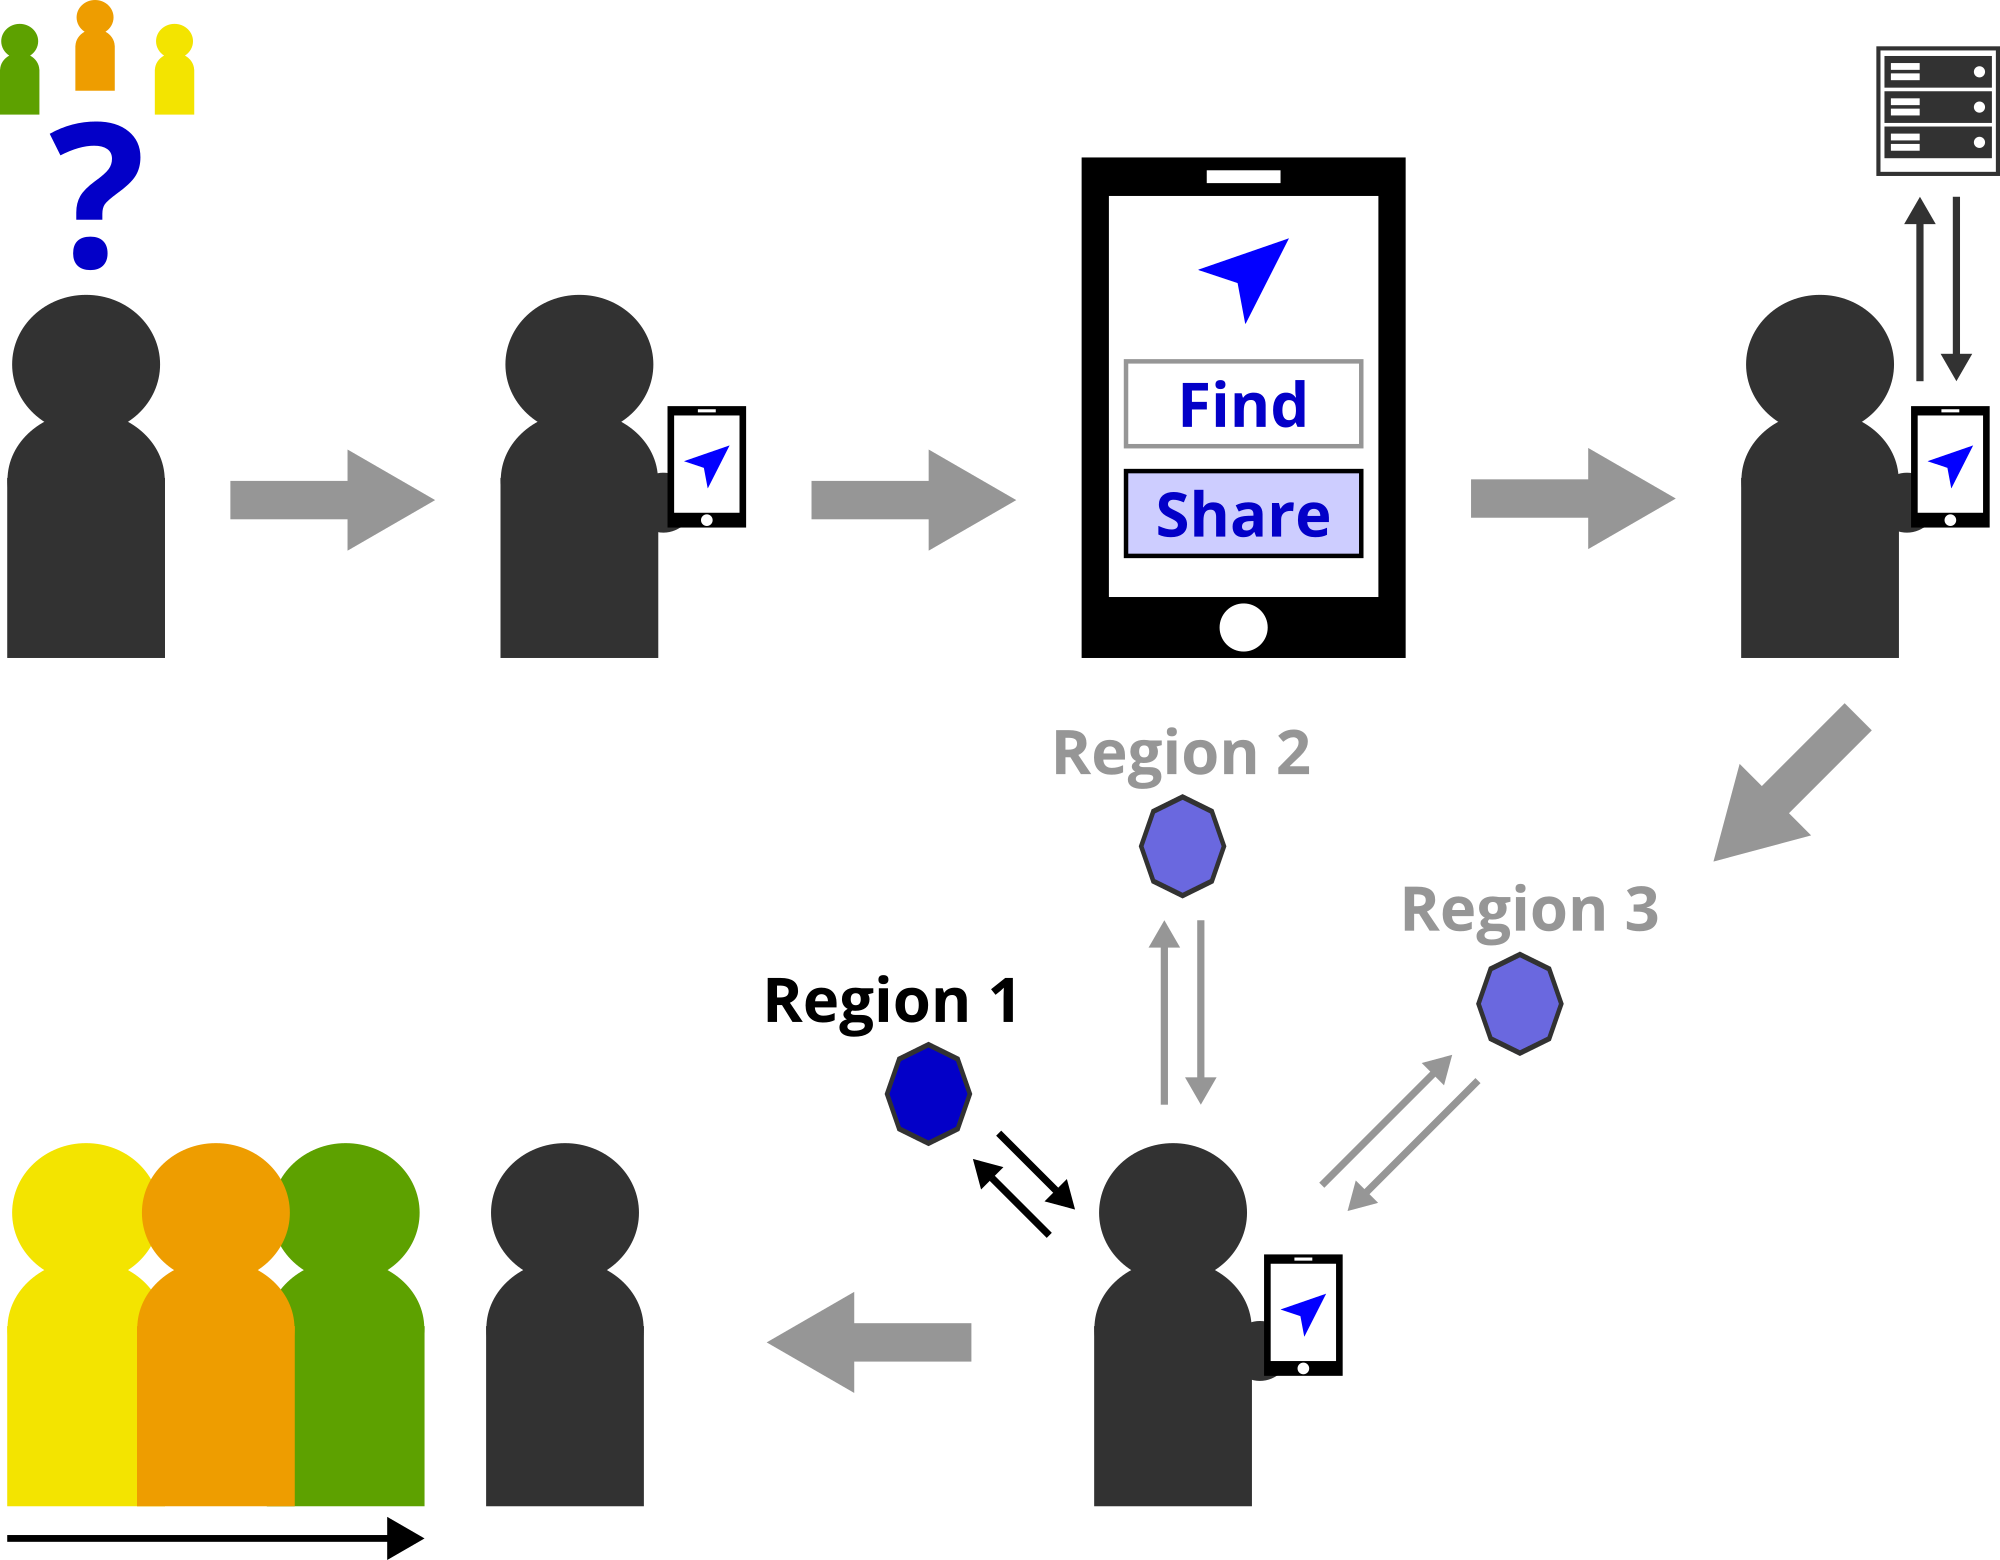
\includegraphics[width=\textwidth]{user-story}\\
    Steps on user's way to her/his friends.
\end{center}


\section{Constraints}

The idea of this project described above already introduced some implicit constraints in order to make it work. To have a complete overview of what we expect to have available to use our service, we defined the following constraints:

\begin{itemize}
    \item \textbf{Everyone has a smartphone}: As this project involves developing clients for Android and iOS and relying on these clients to interact in an user friendly manner with the backend, a smartphone is needed. We do not, though, require the latest operating system versions. For Android, version 5.0 is required, for iOS, version 9 is required.
    \item \textbf{Participants have a TUB account (edugain account)}: The service we provide needs an authentication prior to being able to modify or delete objects on backend side. Therefore some kind of user management was needed. As we will explain more deeply later in this document, for user authentication and session management we rely on a department service called CYCLONE Federation Provider\footnote{\url{http://www.cyclone-project.eu/}}. Via this service users with an edugain (and therefore a TUB) account are able to authenticate against our backend.
    \item \textbf{Minimal interaction}: As described in the previous section our intended use case is placed in situations where you probably carry a tray full of food and will not be having your hands free to interact with complex user interfaces. Therefore a very important constraint for our project was to provide applications that do not need a lot of intention in order to work as intended while at the same time strictly comply with the user's set preferences.
    \item \textbf{Easy to use}: This constraint correlates with the previous one. The setting our applications are intended for do not allow for complex user interfaces. Actions needed to be taken while using the services need to be easy to perform.
    \item \textbf{Low impact on device battery}: The possible use of bluetooth introduced the topic of battery usage. We therefore defined low battery usage as an important constraint for our project.
\end{itemize}


\vspace{0.5cm}

\section{Functional Requirements}

After motivation and constraints were set, we defined our functional requirements. These were the functions we had to implement to follow along our imagined flow throughout the application. Therefore a user has to be able to\ldots

\begin{itemize}
    \item \textbf{\ldots login via university account}: As mentioned in our constraints, login should happen via the university account. We are using the CYCLONE Federation Provider and therefore things work a little different than in a self-developed login mechanism. For us this meant to integrate the provided OpenID Connect authentication flow in a user friendly way into the mobile applications. The applications in turn would then be authenticated against the backend.
    \item \textbf{\ldots add friends via university mail}: All connected edugain members each have their own unique domain name and internally only contain unique users. It was the logical step to provide the functionality to add friends by their mail address as the unique identifier.
    \item \textbf{\ldots share her/his location}: The most important part of our system is the modifiability of the logged in user only. This includes updating or deleting the user's location and defining in which conditions and with which friends the location should be shared.
    \item \textbf{\ldots see shared locations of friends}: Friend's locations were supposed to be visualized on a map. To realise this a functionality to retrieve locations of friends directly in the user's area needed to be developed.
\end{itemize}
